Here is an example of cool tables.

\begin{table}[ht]
\caption{Example table with math and verbatim texts.}
\label{tab:jacobi}
\centering
\renewcommand{\arraystretch}{1.5}
\begin{tabular}{c:l}\hline
\textbf{System} & \hspace{0.1cm}\textbf{Representation} \\\hline
\cellcolor{TableRowColor}Rendered Version & \cellcolor{TableRowColor}\hspace{0.1cm}$P_n^{(\alpha, \beta)}(\cos(a\Theta))$ \\
Generic \LaTeX & \hspace{0.1cm}\small\verb|P_n^{(\alpha, \beta)}(\cos(a\Theta))| \\
\cellcolor{TableRowColor}Semantic \LaTeX & \cellcolor{TableRowColor}\hspace{0.1cm}\small \verb|\JacobipolyP{\alpha}{\beta}{n}@{\cos@{a\Theta}}| \\
Maple & \hspace{0.1cm}\small\verb|JacobiP(n, alpha, beta, cos(a*Theta))| \\
\cellcolor{TableRowColor}Mathematica & \cellcolor{TableRowColor}\hspace{0.1cm}\small \verb|JacobiP[n, \[Alpha], \[Beta], Cos[a \[CapitalTheta]]]| \\
SymPy & \hspace{0.1cm}\footnotesize\verb|jacobi(n,Symbol('alpha'),Symbol('beta'),cos(a*Symbol('Theta')))| \\\hline
\end{tabular}
\end{table}

\begin{table}[ht]
\caption[Short caption for LOTs.]{Table with colorful ticks and crosses.}
\label{tab:tex-cas-translations}
\centering
\renewcommand{\arraystretch}{1.3}
\begin{tabular}{l;{1pt/1pt}c:c:c:c:c:c}\hline
	\multicolumn{1}{c:}{\textbf{\LaTeX}} & \textbf{Rendering} & \texttt{MM} & \texttt{SP} & \texttt{ST} & \texttt{WA} & \texttt{LCT}\textsubscript{1} \\\hline
	\rowcolor{TableRowColor}
	\verb|\int_a^b x dx| 			& $\int_a^b x dx$ 			& \crossMark & \checkMark & \crossMark & \checkMark & \crossMark \\
	\verb|\int_a^b x \mathrm{d}x| 	& $\int_a^b x \mathrm{d}x$ & \crossMark & \crossMark & \crossMark & \checkMark & \crossMark \\
	\rowcolor{TableRowColor}
	\verb|\int_a^b x\, dx| 		& $\int_a^b x\, dx$ 		& \checkMark & \checkMark & \crossMark & \checkMark & \crossMark \\
	\verb|\int_a^b x\; dx| 		& $\int_a^b x\; dx$ 		& \crossMark & \checkMark & \crossMark & \checkMark & \crossMark \\
	\rowcolor{TableRowColor}
	\verb|\int_a^b x\, \mathrm{d}x|& $\int_a^b x\, \mathrm{d}x$& \crossMark & \crossMark & \crossMark & \checkMark & \crossMark \\
	\verb|\int_a^b \frac{dx}{x}| 	& $\int_a^b \tfrac{dx}{x}$ & \crossMark & \checkMark & \crossMark & \checkMark & \crossMark \\
	\rowcolor{TableRowColor}
	\verb|\sum_{n=0}^N n^2| 		& $\sum_{n=0}^N n^2$ 		& \checkMark & \checkMark & \checkMark & \checkMark & \checkMark \\
	\verb|\sum_{n=0}^N n^2 + n| 	& $\sum_{n=0}^N n^2 + n$ 	& \questionMark & \questionMark & \crossMark & \questionMark & \questionMark \\
	\rowcolor{TableRowColor}
	\verb|{n \choose m}| 			& $\binom{n}{m}$ 			& \crossMark & \crossMark & \crossMark & \checkMark & \crossMark \\
	\verb|\binom{n}{m}| 			& $\binom{n}{m}$ 			& \checkMark & \checkMark & \checkMark & \checkMark & \checkMark \\
	\rowcolor{TableRowColor}
	
	{\footnotesize\verb|P_n^{(\alpha,\beta)}(\cos(a\Theta))|} & $P_n^{(\alpha,\beta)}(\cos(a\Theta))$ & \checkMark & \crossMark & \crossMark & \crossMark & \checkMark \\
	\verb|\cos(a\Theta)| 			& $\cos(a\Theta)$ 			& \checkMark & \checkMark & \checkMark & \checkMark & \checkMark \\
	\rowcolor{TableRowColor}
	\verb|\frac{d}{dx} \sin(x)| 			& $\frac{d}{dx} \sin(x)$ 			& \crossMark & \checkMark & \crossMark & \checkMark & \crossMark \\
	\hline
\end{tabular}
\end{table}

And a figure.

\begin{figure}[t]
	\centering
	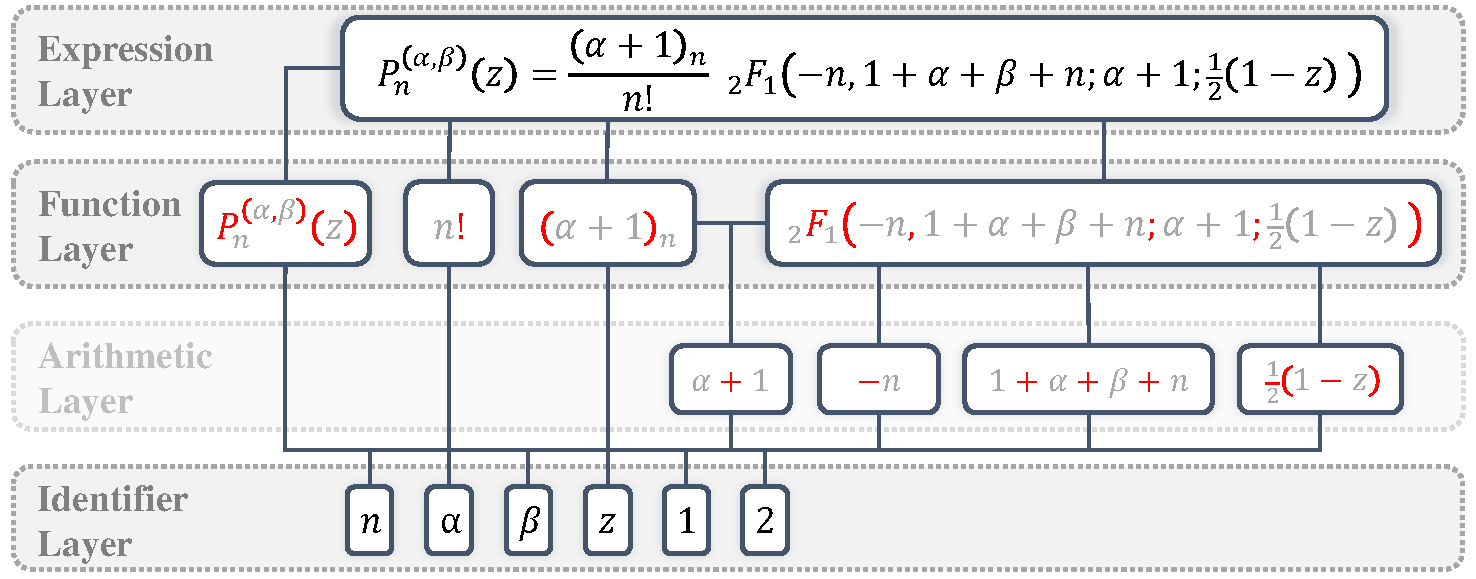
\includegraphics[width=\textwidth]{moi-layers-4L.pdf}
	\caption[Short caption for the List of Figures.]{Long caption directly below the picture.}
	\label{fig:moi-layers-4l}
\end{figure}

\pagebreak
And a lot of different information boxes. Take a look at \verb|boxexample.tex| for further details.

\begin{thesisobjectivebox}
Your thesis objective
\end{thesisobjectivebox}

\begin{researchtaskbox}{Research Tasks Box}
\begin{enumerate}[label=\textbf{\Roman*}, labelsep=1em]
\setlength\itemsep{0.25em}
\item\label{rt:I} \lipsum[1][3]
\item\label{rt:II} \lipsum[1][4]
\item\label{rt:III} \lipsum[1][5]
\item\label{rt:IV} \lipsum[1][6]
\item\label{rt:V} \lipsum[1][7]
\end{enumerate}
\end{researchtaskbox}

\begin{infobox}{Small Icon Info Box}
With additional infos.
\end{infobox}

\begin{examplebox}{Example Box}
With an example
\end{examplebox}

\begin{examplebox}{Single Line Info Box: \normalfont\mdseries With normal font following.}
\vspace*{-0.165cm}
\end{examplebox}

\paperbox{Www20-frontpage.jpg}{%
\textit{``Discovering Mathematical Objects of Interest --- A Study of Mathematical Notations''} by \textbf{Andr\'{e} Greiner-Petter}, Moritz Schubotz, Fabien M\"{u}ller, Corinna Bretinger, Howard S.~Cohl, Akiko Aizawa, and Bela Gipp. \textbf{In:} \textit{Proceedings of the Web Conference} (WWW), 2020.%
}{Chapter~\ref{ch:related-work} --- \cite{GreinerPetterSMB20}}

\begin{definitionbox}{Definition Box}[def:caption]
A nice definition box.
\end{definitionbox}

\begin{translationbox}{Translation Box}
Usually you want nice code box inside, see the next box as an example.
\end{translationbox}

\begin{translationbox}{Translation Box with Code}
\begin{code}[mytex]
P_n^{(\alpha,\beta)}(z) = \frac{(\alpha+1)_n}{n!} {}_2F_1\left(-n,1+\alpha+\beta+n;\alpha+1;\tfrac{1}{2}(1-z)\right)
\end{code}
\end{translationbox}

\begin{translationbox}{Translation Box with Custom Code}
\begin{customcode}[language=maple, mathescape=false]
diff( exp(z^2)*erfc(z), [z$(n)] ) = (-1)^(n)*(2)^(n)*factorial(n)*exp(z^2)*erfc(n, z)
\end{customcode} %$ %fool editor that the equation is "closed"
\vspace{-0.2cm}
\begin{footnotesize}
\vspace{-0.15cm}
\hfill Redundant parentheses removed to improve readability.
\end{footnotesize}
\end{translationbox}

\begin{translationbox}{Translation of Bailey’s Transformation of Very-Well-Poised ${}_{8}\phi_{7}$}
\begin{customcode}[language=mymathematica, basicstyle=\LSTfont, numbers=none, stepnumber=1, numbersep=6pt]
QHypergeometricPFQ[{a, q*(a)^(Divide[1,2]),-q*(a)^(Divide[1,2]),b,c,d,e,f},{(a)^(Divide[1,2]), -(a)^(Divide[1,2]),a*q/b,a*q/c,a*q/d,a*q/e,a*q/f},q, Divide[(a)^(2)*(q)^(2),b*c*d*e*f]] 
 == Divide[Product[QPochhammer[Part[{a*q,a*q/(d*e),a*q/(d*f),a*q/(e*f)},i],q, Infinity],{i,1, Length[{a*q,a*q/(d*e),a*q/(d*f),a*q/(e*f)}]}], Product[QPochhammer[Part[{a*q/d,a*q/e,a*q/f,a*q/(d*e*f)},i],q, Infinity],{i,1, Length[{a*q/d,a*q/e,a*q/f,a*q/(d*e*f)}]}]]* QHypergeometricPFQ[{a*q/(b*c),d,e,f},{a*q/b,a*q/c,d*e*f/a},q,q]
 + Divide[Product[QPochhammer[Part[{a*q,a*q/(b*c),d,e,f,(a)^(2)*(q)^(2)/(b*d*e*f),(a)^(2)*(q)^(2)/(c*d*e*f)},i],q, Infinity],{i,1, Length[{a*q,a*q/(b*c),d,e,f,(a)^(2)*(q)^(2)/(b*d*e*f),(a)^(2)*(q)^(2)/(c*d*e*f)}]}], Product[QPochhammer[Part[{a*q/b,a*q/c,a*q/d,a*q/e,a*q/f,(a)^(2)*(q)^(2)/(b*c*d*e*f),d*e*f/(a*q)},i],q, Infinity],{i,1, Length[{a*q/b,a*q/c,a*q/d,a*q/e, a*q/f,(a)^(2)*(q)^(2)/(b*c*d*e*f),d*e*f/(a*q)}]}]]
 * QHypergeometricPFQ[{a*q/(d*e),a*q/(d*f), a*q/(e*f),(a)^(2)*(q)^(2)/(b*c*d*e*f)},{(a)^(2)*(q)^(2)/(b*d*e*f),(a)^(2)*(q)^(2)/(c*d*e*f), a*(q)^(2)/(d*e*f)},q,q]
\end{customcode}
\vspace{-0.35cm}
\begin{footnotesize}
\hfill\rule{0.4\textwidth}{.4pt}

\vspace{-0.15cm}
\hfill Linebreaks are manually added to improve readability.
\end{footnotesize}
\end{translationbox}

\begin{codebox}{A Code Box}
\begin{code}[MathML]
<mrow>
  <msub>
    <mi>P</mi>
    <mi>n</mi>
  </msub>
  <mo>
    <!-- Invisible 
    Funct. Appl. 
    Unicode U+2061 -->  
  </mo>
  <mrow>
    <mo>(</mo>
    <mi>x</mi>
    <mo>)</mo>
  </mrow>
</mrow>
\end{code}
\end{codebox}

\begin{codebox}{A Code Box With Caption}[With Caption Text][code:caption]
\begin{code}[MathML]
<mrow></mrow>
\end{code}
\end{codebox}

\begin{codebox}{A Latex Code Box}[With caption.][lst:caption]
\begin{code}[mytex]
P_n^{(\alpha , \beta)}(x)          % Generic LaTeX
\JacobipolyP{n}{\alpha}{\beta}@{x} % Semantic LaTeX
\end{code}
\end{codebox}
